%\documentclass{layout/tudelft-aiaa}
\documentclass[twocolumn]{tudelft-aiaa}

%% Additional packages
\usepackage[T1]{fontenc}
\usepackage[utf8]{inputenc}

\usepackage{xcolor}
\usepackage{courier}
\usepackage{xfrac}


% Wordle colors
\definecolor{k}{RGB}{121,124,126}
\definecolor{y}{RGB}{195,180,95}
\definecolor{g}{RGB}{129,170,105}

\usepackage{graphicx} % Adding images
\usepackage{amsmath} % Mathematics
\usepackage{siunitx} % Various functions, e.g. \num{}
\usepackage{tabularx} % Additional functions to tables
\usepackage{subcaption} % Subfigures and subcaptions

%% Additional commands
\setlength{\nomitemsep}{-\parsep} % Reduce white space in nomenclature
\setlength{\bibsep}{1pt} % Reduce white space in references
\renewcommand{\deg}{\si{\degree}\xspace}

%%%%% Title %%%%%

\title{Solving Wordle Heuristically \normalsize \color{red} \emph{(DRAFT --- \today}) \color{black}}

\author{\textbf{Daniel W. Dichter}}
\affil{Independent Researcher\\Cambridge, Massachusetts, U.S.A.\\daniel.w.dichter@gmail.com}

\begin{document}

\AlwaysPagewidth{

\maketitle

%%%%% Abstract %%%%%

\begin{abstract}
\noindent \normalfont Wordle is a daily word game in which a player must guess a hidden five-letter word in six or fewer tries. After each guess, they get a color-coded response that indicates how close their guess was. This paper describes a solver that wins all 2,315 possible games, averaging a score of 3.692 with a standard deviation of 0.734. This is comparable to the current best solvers known, yet is achieved heuristically with many fewer calculations.

\end{abstract}

\vspace{3 mm}

}

%%%%% Main Body %%%%%

\section{Game Parameters}

Wordle has two dictionaries: 2,315 possible solutions, and 12,972 acceptable guesses.\cite{Wardle}\cite{Glaiel} Solutions are limited to commonly-known, non-S-plural words. The default version of the game is assumed, wherein guesses need not be consistent with known information. Games are assumed to be mutually independent, and thereby the solver cannot recall previous solutions to reduce the set of initial words.

\section{Eliminating Solutions}

After each guess, some solutions can be eliminated. This is executed sequentially, tile-by-tile, as follows.

\emph{Gray tile.} If any and all additional letter-matching tiles are also gray, eliminate words that contain this letter. Otherwise, eliminate words that contain this letter in this position, and eliminate words that do not contain the overall quantity of this letter indicated.

\emph{Yellow tile.} Eliminate words that contain this letter in this position, and eliminate words that do not contain this letter in non-green non-letter-matching tiles.

\emph{Green tile.} Eliminate words that do not contain this letter in this position.

\section{Probability and Value Matrices}

At any game state, a matrix measuring 26 x 5 may be defined that reports the probability of each letter in each position of the solution.

Guessing a tile with zero or unity probability\footnote{Obtained directly by a gray or green tile, or indirectly by deduction.} provides no information. This observation is generalized by stating that "bad" guesses have high certainty. It follows that "good" guesses have low certainity, which is equivalent to intermediate probability. This is formalized as transfer function relating probability $P$ to value $V$, modeled as one period of a sine function with $V(P=0,1)=0$ and $V(P=\sfrac{1}{2})=1$. Gaussian and triangular functions intersecting these same $(P,V)$ points with equal $\text{sign}(dP/dV)$ were found to perform marginally worse.

Another matrix, also measuring 26 x 5, may then be defined that reports the value of each letter in each position of the solution.

\begin{table}[h!]
\begin{centering}
\begin{tabular}{l r}
\bf{Game State} & \bf{Words Left}\\
\hline
\noindent \vspace{1 mm} \texttt{\textcolor{white}{\textbf{\colorbox{g}{S}\hspace{1 mm}\colorbox{k}{O}\hspace{1 mm}\colorbox{k}{A}\hspace{1 mm}\colorbox{k}{R}\hspace{1 mm}\colorbox{k}{E}\hspace{1 mm}}}} & 2,315\\
\noindent \vspace{1 mm} \texttt{\textcolor{white}{\textbf{\colorbox{k}{F}\hspace{1 mm}\colorbox{y}{L}\hspace{1 mm}\colorbox{g}{I}\hspace{1 mm}\colorbox{k}{N}\hspace{1 mm}\colorbox{k}{T}\hspace{1 mm}}}} & 63\\
\noindent \vspace{1 mm} \texttt{\textcolor{white}{\textbf{\colorbox{k}{A}\hspace{1 mm}\colorbox{k}{P}\hspace{1 mm}\colorbox{k}{E}\hspace{1 mm}\colorbox{k}{A}\hspace{1 mm}\colorbox{y}{K}\hspace{1 mm}}}} & 3\\
\noindent \vspace{1 mm} \texttt{\textcolor{white}{\textbf{\colorbox{g}{S}\hspace{1 mm}\colorbox{g}{K}\hspace{1 mm}\colorbox{g}{I}\hspace{1 mm}\colorbox{g}{L}\hspace{1 mm}\colorbox{g}{L}\hspace{1 mm}}}} & 1\\
\hline
\noindent \vspace{1 mm} \texttt{\textcolor{white}{\textbf{\colorbox{k}{S}\hspace{1 mm}\colorbox{y}{O}\hspace{1 mm}\colorbox{y}{A}\hspace{1 mm}\colorbox{k}{R}\hspace{1 mm}\colorbox{k}{E}\hspace{1 mm}}}} & 2,315\\
\noindent \vspace{1 mm} \texttt{\textcolor{white}{\textbf{\colorbox{g}{A}\hspace{1 mm}\colorbox{g}{L}\hspace{1 mm}\colorbox{g}{O}\hspace{1 mm}\colorbox{g}{F}\hspace{1 mm}\colorbox{g}{T}\hspace{1 mm}}}} & 44\\
\hline
\noindent \vspace{1 mm} \texttt{\textcolor{white}{\textbf{\colorbox{k}{S}\hspace{1 mm}\colorbox{k}{O}\hspace{1 mm}\colorbox{y}{A}\hspace{1 mm}\colorbox{k}{R}\hspace{1 mm}\colorbox{y}{E}\hspace{1 mm}}}} & 2,315\\
\noindent \vspace{1 mm} \texttt{\textcolor{white}{\textbf{\colorbox{g}{P}\hspace{1 mm}\colorbox{y}{E}\hspace{1 mm}\colorbox{y}{T}\hspace{1 mm}\colorbox{g}{A}\hspace{1 mm}\colorbox{y}{L}\hspace{1 mm}}}} & 68\\
\noindent \vspace{1 mm} \texttt{\textcolor{white}{\textbf{\colorbox{g}{P}\hspace{1 mm}\colorbox{g}{L}\hspace{1 mm}\colorbox{g}{E}\hspace{1 mm}\colorbox{g}{A}\hspace{1 mm}\colorbox{g}{T}\hspace{1 mm}}}} & 1\\
\hline
\noindent \vspace{1 mm} \texttt{\textcolor{white}{\textbf{\colorbox{g}{S}\hspace{1 mm}\colorbox{k}{O}\hspace{1 mm}\colorbox{g}{A}\hspace{1 mm}\colorbox{g}{R}\hspace{1 mm}\colorbox{k}{E}\hspace{1 mm}}}} & 2,315\\
\noindent \vspace{1 mm} \texttt{\textcolor{white}{\textbf{\colorbox{k}{T}\hspace{1 mm}\colorbox{g}{H}\hspace{1 mm}\colorbox{g}{A}\hspace{1 mm}\colorbox{k}{C}\hspace{1 mm}\colorbox{k}{K}\hspace{1 mm}}}} & 11\\
\noindent \vspace{1 mm} \texttt{\textcolor{white}{\textbf{\colorbox{g}{S}\hspace{1 mm}\colorbox{g}{H}\hspace{1 mm}\colorbox{g}{A}\hspace{1 mm}\colorbox{g}{R}\hspace{1 mm}\colorbox{g}{D}\hspace{1 mm}}}} & 2\\
%\hline
%\noindent \vspace{1 mm} \texttt{\textcolor{white}{\textbf{\colorbox{y}{S}\hspace{1 mm}\colorbox{g}{O}\hspace{1 mm}\colorbox{k}{A}\hspace{1 mm}\colorbox{k}{R}\hspace{1 mm}\colorbox{k}{E}\hspace{1 mm}}}} & 2,315\\
%\noindent \vspace{1 mm} \texttt{\textcolor{white}{\textbf{\colorbox{k}{B}\hspace{1 mm}\colorbox{k}{U}\hspace{1 mm}\colorbox{g}{I}\hspace{1 mm}\colorbox{g}{S}\hspace{1 mm}\colorbox{g}{T}\hspace{1 mm}}}} & 15\\
%\noindent \vspace{1 mm} \texttt{\textcolor{white}{\textbf{\colorbox{k}{F}\hspace{1 mm}\colorbox{k}{E}\hspace{1 mm}\colorbox{k}{H}\hspace{1 mm}\colorbox{y}{M}\hspace{1 mm}\colorbox{k}{E}\hspace{1 mm}}}} & 4\\
%\noindent \vspace{1 mm} \texttt{\textcolor{white}{\textbf{\colorbox{g}{M}\hspace{1 mm}\colorbox{g}{O}\hspace{1 mm}\colorbox{g}{I}\hspace{1 mm}\colorbox{g}{S}\hspace{1 mm}\colorbox{g}{T}\hspace{1 mm}}}} & 1\\
\end{tabular}
\vspace{2 mm}
\caption{Solutions for recent games.}
\label{table_games}
\end{centering}
\end{table}

\section{Scoring and Guessing}

After every guess, the value matrix is updated per the remaining solutions and used to score all guesses. Scoring is also executed sequentially, tile-by-tile. Interactions between tiles are modeled with a set of heuristics, as follows.

A tile with non-unity probability captures the value of that letter in that position, and one-half the value of that letter in all other positions; with unity probability it captures no value in any position. Guesses with multiple tiles of the same letter interfere with each other; their value capture is equal to their nominal sum divided by their quantity, excepting letter-matching unity-probability tiles. Guesses where the quantity of letter-matching tiles is less than or equal to the quantity of unity-probability letter-matching tiles may refer back to the unity-probability tile(s) as yellow; tiles matching this condition are diminished in value by a factor of one-half.

The top-scoring word is picked until there are two or fewer solutions remaining. Ties are broken first by solution probability, then alphabetically.

\pagebreak

\section{Results}

Top-scoring first words are shown in Table \ref{table_words}. Solutions for recent games are shown in Table \ref{table_games}. Results for all games are shown in Table \ref{table_results}. A comparison with other solvers including unassisted play by proxy of Twitter\footnote{29 unique games, 7,087,784 tweets total.} is shown in Table \ref{other_solvers} and Figure \ref{performance_comparison}.\cite{WordleStats} Source code and complete game logs are also provided.\cite{Dichter}

\section{Discussion}

All games are opened with the top-scoring word \texttt{SOARE}. In the middlegame, emergent strategies can be seen, such as abandoning green tiles until the endgame, shifting yellow tiles to alternate positions, and reusing gray tiles for high-value words. The cumulative density function (CDF) shows that 88.5\% of games are won within four moves, 99.0\% within five, and 100\% within six. The probability density function (PDF) shows a mode of four moves, with an associated probability of 47.9\%. The average score is within 7\% of the current best solvers known, which are substantially more complex and/or computationally expensive. An average score lower limit of about 3.5 is theorized based on the maximum amount of information that may be obtained in the first two moves.\cite{Sanderson}

\section{Acknowledgments}

The author gratefully thanks Jess Hall, Julius Dichter, Adam Filion, and Tyler Smith for their support.

\begin{table}[h!]
\begin{centering}
\begin{tabular}{ r | l | l}
\bf Rank & \bf Word & \bf Score\\
\hline
1  & \texttt{SOARE} & 1.00000\\
2  & \texttt{STARE} & 0.93367\\
3  & \texttt{SAINE} & 0.92580\\
4  & \texttt{SAICE} & 0.91265\\
5  & \texttt{SLATE} & 0.91234\\
6  & \texttt{RAISE} & 0.91178\\
7  & \texttt{AROSE} & 0.91162\\
8  & \texttt{SNARE} & 0.90631\\
9  & \texttt{ARISE} & 0.90500\\
10 & \texttt{STOAE} & 0.90352\\
\end{tabular}
\vspace{2 mm}
\caption{Top-scoring first words.}
\label{table_words}
\end{centering}
\end{table}

\begin{table}[h!]
\begin{centering}
\begin{tabular}{ r | r | l | l}
\bf Score & \bf Games & \bf PDF & \bf CDF\\
\hline
1 & 0 & 0.000 & 0.000\\
2 & 63 & 0.027 & 0.027\\
3 & 876 & 0.378 & 0.406\\
4 & 1,110 & 0.479 & 0.885\\
5 & 242 & 0.105 & 0.990\\
6 & 24 & 0.010 & 1.000\\
x & 0 & 0.000 & 1.000\\
\end{tabular}
\vspace{2 mm}
\caption{Results for all games.}
\label{table_results}
\end{centering}
\end{table}

\begin{figure}[h!]
  \centering
    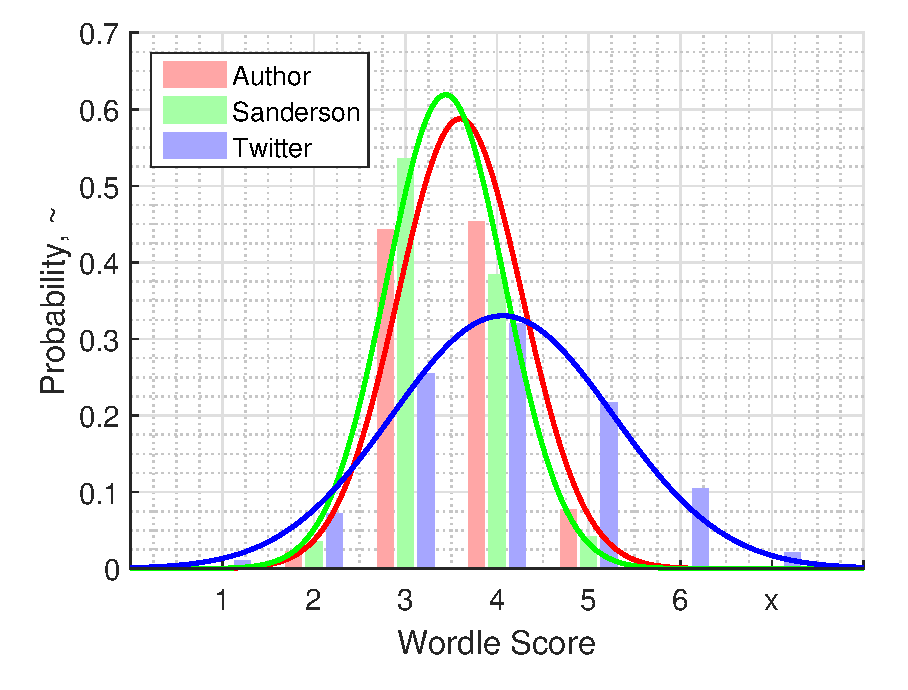
\includegraphics[width=0.5\textwidth]{performance_comparison.eps}
  \caption{Comparison of solver distributions.}
\label{performance_comparison}
\end{figure}

\begin{table}[h!]
\begin{centering}
\setlength\tabcolsep{3pt} % default value: 6pt
\begin{tabular}{l | r | r | r | r | l}
\bf Solver & \bf Win \% & \bf Mean & \bf Stdev. & \bf Worst & \bf Opener\\
\hline \hline
Author\cite{Dichter} & 100.0 & 3.692 & 0.734 & 6 & \texttt{SOARE}\\ \hline
Sanderson\cite{Sanderson} & 100.0 & 3.438 & 0.645 & 6 & \texttt{CRANE}\\
Glaiel\cite{Glaiel} & 100.0 & 3.494 & - & 5 & \texttt{ROATE}\\
Chao\cite{Chao} & 99.7 & 3.420 & - & x & \texttt{OPERA}\\
Filion\cite{Filion} & 94.2 & - & - & x & \texttt{AROSE}\\
Twitter\cite{WordleStats} & 97.9 & 4.061 & 1.208 & x & \texttt{-}\\
\end{tabular}
\vspace{2 mm}
\caption{Comparison of solver benchmarks.}
\label{other_solvers}
\end{centering}
\end{table}

%%%%% Bibliography %%%%%

%\renewcommand{\bibpreamble}{For a full documentation of the references, please refer to the sample.bib file. You can delete this text/command safely in main.tex at line 73. \cite{example-article,example-article-published-online,example-inbook,example-inbook-series-with-editor,example-inproceedings,example-proceedings,example-report,example-paper,example-phdthesis}}

\raggedright

\bibliography{article}

\begin{thebibliography}{9}

\bibitem{Wardle}
Wardle, Josh. \emph{Wordle - a daily word game.} Accessed February 6, 2022. https://www.powerlanguage.co.uk/wordle/.

\bibitem{Glaiel}
Glaiel, Tyler. \emph{The mathematically optimal first guess in Wordle.} Accessed February 6, 2022. https://medium.com/@tglaiel/the-mathematically-optimal-first-guess-in-wordle-cbcb03c19b0a.

\bibitem{WordleStats}
O'Connor, Kevin. \emph{Wordle Stats (@WordleStats) / Twitter.} Accessed February 6, 2022. https://twitter.com/wordlestats.

\bibitem{Dichter}
Dichter, Daniel. \emph{wordle\_solver.} Accessed February 6, 2022. https://github.com/kindofdoon/wordle\_solver.

\bibitem{Sanderson}
Sanderson, Grant. \emph{The mathematically optimal Wordle strategy.} 3Blue1Brown. Accessed February 6, 2022. https://www.youtube.com/watch?v=v68zYyaEmEA.

\bibitem{Chao}
Chao, Jason. \emph{Wordle-Solver.} Accessed February 6, 2022. https://github.com/jason-chao/wordle-solver.

\bibitem{Filion}
Filion, Adam. \emph{Building a Wordle Solver.} Accessed February 6, 2022. https://blogs.mathworks.com/loren/2022/01/18/building-a-wordle-solver/.

\end{thebibliography}

\end{document}













